% Slide 1
\begin{frame}
    \frametitle{Normal Form Games}

    \centering
    \( \overbrace{
    \begin{tikzpicture}[node/.style={draw, circle}]
        \node[draw=none] (first) at (0,0) {\Strichmaxerl[3]};
        \node[draw=none] (second) at (2,0) {\Strichmaxerl[3]};
        \node[draw=none] (third) at (4,0) {\Strichmaxerl[3]};
        \node[draw=none] (dots) at (6,0) {\(\dots\)};
        \node[draw=none] (last) at (8,0) {\Strichmaxerl[3]};

        \node[draw=none] (action_1) at (-0.4, -3) {};
        \node[draw=none] (action_2) at (0.4, -3) {};
        \node[draw=none] (action_3) at (1.6, -3) {};
        \node[draw=none] (action_4) at (2.4, -3) {};
        \node[draw=none] (action_5) at (3.25, -3) {};
        \node[draw=none] (action_6) at (4, -3) {};
        \node[draw=none] (action_7) at (4.75, -3) {};
        \node[draw=none] (action_8) at (7.6, -3) {};
        \node[draw=none] (action_9) at (8.4, -3) {};

    \end{tikzpicture}
    }^{\textbf{N players}} \)
\end{frame}

% Slide 2
\begin{frame}
    \frametitle{Normal Form Games}

    \centering
    \(\overbrace{
    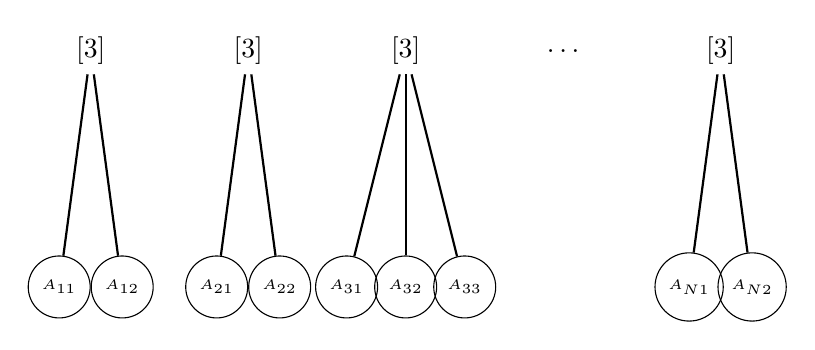
\begin{tikzpicture}[node/.style={draw, circle}]
        \node[draw=none] (first) at (0,0) {\Strichmaxerl[3]};
        \node[draw=none] (second) at (2,0) {\Strichmaxerl[3]};
        \node[draw=none] (third) at (4,0) {\Strichmaxerl[3]};
        \node[draw=none] (dots) at (6,0) {\(\dots\)};
        \node[draw=none] (last) at (8,0) {\Strichmaxerl[3]};

        \node[node] (action_1) at (-0.4, -3) {\tiny{$A_{11}$}};
        \node[node] (action_2) at (0.4, -3) {\tiny{$A_{12}$}};
        \node[node] (action_3) at (1.6, -3) {\tiny{$A_{21}$}};
        \node[node] (action_4) at (2.4, -3) {\tiny{$A_{22}$}};
        \node[node] (action_5) at (3.25, -3) {\tiny{$A_{31}$}};
        \node[node] (action_6) at (4, -3) {\tiny{$A_{32}$}};
        \node[node] (action_7) at (4.75, -3) {\tiny{$A_{33}$}};
        \node[node] (action_8) at (7.6, -3) {\tiny{$A_{N1}$}};
        \node[node] (action_9) at (8.4, -3) {\tiny{$A_{N2}$}};

        \draw [thick] (first) -- (action_1);
        \draw [thick] (first) -- (action_2);
        \draw [thick] (second) -- (action_3);
        \draw [thick] (second) -- (action_4);
        \draw [thick] (third) -- (action_5);
        \draw [thick] (third) -- (action_6);
        \draw [thick] (third) -- (action_7);
        \draw [thick] (last) -- (action_8);
        \draw [thick] (last) -- (action_9);
    \end{tikzpicture}
    }^{\textbf{N players}}\)
\end{frame}



% Slide 3
\begin{frame}
    \frametitle{Normal Form Games}

    \centering
    \(\overbrace{
    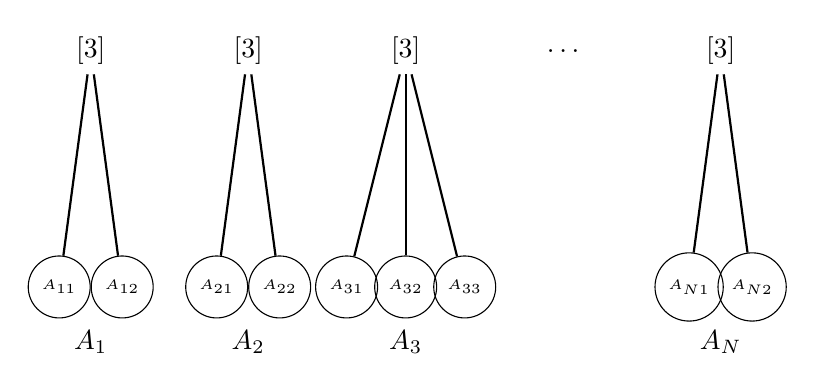
\begin{tikzpicture}[node/.style={draw, circle}]
        \node[draw=none] (first) at (0,0) {\Strichmaxerl[3]};
        \node[draw=none] (second) at (2,0) {\Strichmaxerl[3]};
        \node[draw=none] (third) at (4,0) {\Strichmaxerl[3]};
        \node[draw=none] (dots) at (6,0) {\(\dots\)};
        \node[draw=none] (last) at (8,0) {\Strichmaxerl[3]};

        \node[node] (action_1) at (-0.4, -3) {\tiny{$A_{11}$}};
        \node[node] (action_2) at (0.4, -3) {\tiny{$A_{12}$}};
        \node[node] (action_3) at (1.6, -3) {\tiny{$A_{21}$}};
        \node[node] (action_4) at (2.4, -3) {\tiny{$A_{22}$}};
        \node[node] (action_5) at (3.25, -3) {\tiny{$A_{31}$}};
        \node[node] (action_6) at (4, -3) {\tiny{$A_{32}$}};
        \node[node] (action_7) at (4.75, -3) {\tiny{$A_{33}$}};
        \node[node] (action_8) at (7.6, -3) {\tiny{$A_{N1}$}};
        \node[node] (action_9) at (8.4, -3) {\tiny{$A_{N2}$}};

        \draw [thick] (first) -- (action_1);
        \draw [thick] (first) -- (action_2);
        \draw [thick] (second) -- (action_3);
        \draw [thick] (second) -- (action_4);
        \draw [thick] (third) -- (action_5);
        \draw [thick] (third) -- (action_6);
        \draw [thick] (third) -- (action_7);
        \draw [thick] (last) -- (action_8);
        \draw [thick] (last) -- (action_9);

        \node[draw=none] (action_set_1) at (0, -3.7) {$A_1$};
        \node[draw=none] (action_set_2) at (2, -3.7) {$A_2$};
        \node[draw=none] (action_set_3) at (4, -3.7) {$A_3$};
        \node[draw=none] (action_set_N) at (8, -3.7) {$A_N$}; 
    \end{tikzpicture}
    }^{\textbf{N players}}\)
\end{frame}




% Slide 4
\begin{frame}
    \frametitle{Normal Form Games}

    \centering
    \(\overbrace{
    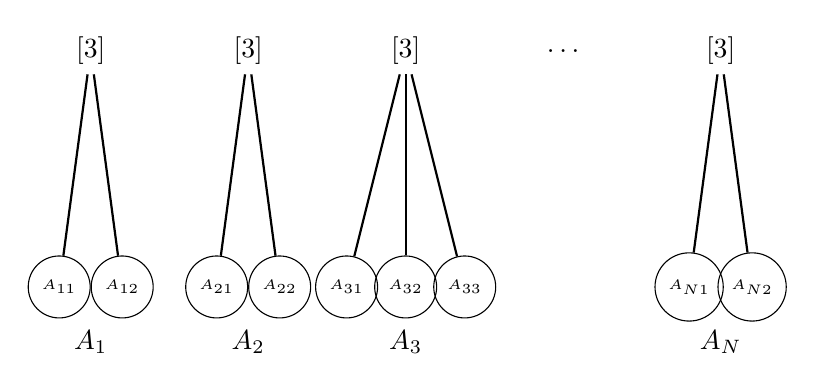
\begin{tikzpicture}[node/.style={draw, circle}]
        \node[draw=none] (first) at (0,0) {\Strichmaxerl[3]};
        \node[draw=none] (second) at (2,0) {\Strichmaxerl[3]};
        \node[draw=none] (third) at (4,0) {\Strichmaxerl[3]};
        \node[draw=none] (dots) at (6,0) {\(\dots\)};
        \node[draw=none] (last) at (8,0) {\Strichmaxerl[3]};

        \node[node] (action_1) at (-0.4, -3) {\tiny{$A_{11}$}};
        \node[node] (action_2) at (0.4, -3) {\tiny{$A_{12}$}};
        \node[node] (action_3) at (1.6, -3) {\tiny{$A_{21}$}};
        \node[node] (action_4) at (2.4, -3) {\tiny{$A_{22}$}};
        \node[node] (action_5) at (3.25, -3) {\tiny{$A_{31}$}};
        \node[node] (action_6) at (4, -3) {\tiny{$A_{32}$}};
        \node[node] (action_7) at (4.75, -3) {\tiny{$A_{33}$}};
        \node[node] (action_8) at (7.6, -3) {\tiny{$A_{N1}$}};
        \node[node] (action_9) at (8.4, -3) {\tiny{$A_{N2}$}};

        \draw [thick] (first) -- (action_1);
        \draw [thick] (first) -- (action_2);
        \draw [thick] (second) -- (action_3);
        \draw [thick] (second) -- (action_4);
        \draw [thick] (third) -- (action_5);
        \draw [thick] (third) -- (action_6);
        \draw [thick] (third) -- (action_7);
        \draw [thick] (last) -- (action_8);
        \draw [thick] (last) -- (action_9);

        \node[draw=none] (action_set_1) at (0, -3.7) {$A_1$};
        \node[draw=none] (action_set_2) at (2, -3.7) {$A_2$};
        \node[draw=none] (action_set_3) at (4, -3.7) {$A_3$};
        \node[draw=none] (action_set_N) at (8, -3.7) {$A_N$}; 
    \end{tikzpicture}
    }^{\textbf{N players}}\)

    \begin{equation*}
        u_i = A_1 \times A_2 \times A_3 \times \dots \times A_N
    \end{equation*}
\end{frame}


% Slide 5 - Example
\begin{frame}
    \frametitle{Rock-Paper-Scissors}
    
    \centering
    \hspace{1cm}
    \includegraphics[width=.3\textwidth]{Bin/rock-paper-scissors.png} \\
    
    \setlength{\columnsep}{0.1pt}
    \begin{multicols}{2}
        \includegraphics[width=.25\textwidth, angle=270]{Bin/rock-paper-scissors.png}

        \begin{equation*}
            \begin{bmatrix}
                (0,0) & (1,-1) & (-1,1) \\
                & & \\
                (-1,1) & (0,0) & (1,-1) \\
                & & \\
                (1,-1) & (-1,1) & (0,0)
            \end{bmatrix}
        \end{equation*}
    \end{multicols}

\end{frame}